\subsection{Fully Connected Neural Networks}
\label{back:linear}

\acrfull{fcnn} are fundamental networks used in many \acrshort{dl} models. Also called dense or linear networks, they are characterized by all neurons being connected between two layers (see Figure \ref{fig:densenn}). 

In the forward pass, linear layers transform the input data, mapping an input vector to an output vector using learnable parameters. The operation can be defined as follows:
\begin{equation}\label{f:wxb}
    \mathbf{y} = \mathbf{w}x+b
\end{equation}
Here, $x$ is the input vector, \textbf{$w$} is the weight matrix, $b$ is the bias, and \textbf{$y$} is the output vector.

\begin{figure}[!h]
    \centering
    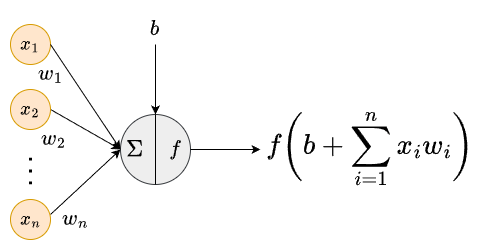
\includegraphics[width=0.7\linewidth]{figures/dl.png}
    \caption{Neurons $x$ in a layer with their weights $w$, a bias $b$ and an activation function $f$}
    \label{fig:dl}
\end{figure}

Furthermore, an activation function $f$ is applied to the output to achieve \textit{nonlinearity}. By applying $f$ to the output $y$, we now get the equation:
\begin{equation}\label{f:fwxb}
    \mathbf{z} = f(\mathbf{y}) = f(\mathbf{w}x+b)
\end{equation}

Some of the more popular activation functions include \cite{szandala2021review}: 

\begin{equation}
    Relu(z) = max(0, z)
\end{equation}

Relu (Rectified Linear Unit) was stated to be the most popular activation function as late as 2018. Its forward and backward pass steps quickly, thus enabling more efficient training compared to other alternatives.

\begin{equation}
    \sigma(z) = \frac{1} {1 + e^{-z}}
\end{equation}

The sigmoid activation is very popular because its range is $[0,1]$, compared to other functions, is rather limited and represents a probabilistic value. This makes it good at outputting probabilistic values.

\begin{equation}
    tanh(x) = \frac{e^x - e^{-x}}{e^x + e^{-x}} = \frac{1 - e^{-2x}}{1 + e^{-2x}}
\end{equation}

Like sigmoid, the hyperbolic tangent has outputs in a relatively small range $[-1, 1]$.

After the forward pass is performed, the network will update its weights. This is done by using a \textit{cost}, or \textit{loss} function and using the resulting loss to calculate the networks' gradients before an optimizer, such as \acrfull{sgd} \cite{Rumelhart1986, Bottou2012}, updates the weights before the following forward pass. For unsupervised networks specifically, two of the more commonly used loss functions include: \\

\textbf{\acrfull{mse}}

\begin{equation}\label{eq:mse}
    \mathcal{L}_{\text{MSE}}(x, \hat{x}) = \dfrac{1}{N}  \sum_{i=1}^{N}(x_i-\hat{x}_i)^2
\end{equation}

The \acrshort{mse} loss function is a commonly used loss function. It punishes bigger differences by squaring the difference between two elements in the prior $x$ and the posterior $\hat{x}$. It then outputs the mean of all the squarred errors computed. \\

\textbf{\acrfull{mae}}

\begin{equation}\label{eq:mae}
    \mathcal{L}_{\text{MAE}}(x, \hat{x}) = \dfrac{1}{N}  \sum_{i=1}^{N}|x_i-\hat{x}_i|
\end{equation}

The \acrshort{mae} loss function is similar to the \acrshort{mse} function. The difference is that the \acrshort{mae} function returns the absolute value of the distance between two distributions $x$ and $\hat{x}$, thus equally punishing all errors. \\

The major bottleneck of all kinds of machine learning techniques is data. The more diverse and varied a . \\

Linear layers have several advantages, such as computational efficiency, flexibility as well as intrerprebility, where the weight and bias vectors can be interpreted as learned parameters. They also serve as building blocks for other components, such as \acrshort{rnn}s \cite{schmidt2019recurrent}, \acrshort{lstm}s \cite{lstm} or even more novel architectures such as the transformer\cite{vaswani2017attention}. \\ 

However, linear layers have several limitations. Due to their inherent linearity, they are prone to \textit{overfitting} and struggle to capture complex relationships in data. This can limit their ability to extract more complex features, potentially reducing some of the model's discriminative power. Furthermore, the size of linear layers can become problematic, especially in \acrshort{fcnn}s. Each neuron connection between layers requires storing weights and biases, which increases the overall model size. For a smaller dense network where the layers are of size $[10, 5, 1]$, the total amount of parameters becomes:
$$\begin{aligned}
S &= (10 \times 5 + 5) + (5 \times 1 + 1) \
&= 50 + 5 + 5 + 1 \
&= 61 \text{ parameters}
\end{aligned}$$
Assuming each parameter is stored as a single-precision floating-point number (\texttt{Float32}, 4 bytes), the total memory size is:
$$\begin{aligned}
\text{Memory size} &= 61 \text{ parameters} \times 4 \text{ bytes/parameter} \
&= 244 \text{ bytes}
\end{aligned}$$ While 244 bytes is small, larger dense networks can quickly consume gigabytes of memory. This can create bottlenecks for hardware accelerators like \acrshort{gpu}s, which typically have less VRAM compared to the \acrshort{ram} available to \acrshort{cpu}s.